\documentclass{article}
\usepackage[letterpaper, margin=1in]{geometry}
\usepackage{ragged2e}
\usepackage[hidelinks]{hyperref}
\usepackage{booktabs}
\usepackage{tabularx}
\usepackage{titling}
\usepackage{setspace}
\usepackage{tikz}
\usepackage{graphicx} % Include graphic importing
\graphicspath{{images/}}
\newcommand{\subtitle}[1]{%
  \posttitle{%
    \par\end{center}
    \begin{center}\large#1\end{center}
    \vskip0.5em}%
}
\usepackage{float}
\usepackage{cite}
\usepackage[toc,nonumberlist,acronym]{glossaries}
\makeglossaries
\newglossaryentry{grist}{name=Grist, text=grist, description="The combination of milled grains to be used in a particular brew. Also sometimes applied to hops \cite{beer-terms}."}
\newglossaryentry{mash}{name=Mash, text=mash, description="(Verb) To release malt sugars by soaking the grains in water. (Noun) The resultant mixture \cite{beer-terms}."}
\newglossaryentry{pitch}{name=Pitch, text=pitch, description="To add yeast."}
\newglossaryentry{sparge}{name=Sparge, text=sparge, description="To spray grist with hot water in order to remove soluble sugars (maltose). This takes place at the end of the mash \cite{beer-terms}."}
\newglossaryentry{trub}{name=Trub, text=trub, description="The layer of sediment that appears at the bottom of the fermentation vessel upon the completion of fermentation."}
\newglossaryentry{wort}{name=Wort, text=wort, description="The solution of grain sugars strained from the mash tun \cite{beer-terms}."}

%\newacronym{abv}{ABV}{Alcohol By Volume}

\author{\\\\}
\title{Brew It Yourself}
\subtitle{An Automated Single-Vessel Home Brewery System}

\begin{document}

\begin{titlepage}
    \begin{center}
        \vspace*{1cm}
        
        \textsc{\LARGE University of Waterloo}\\ [0.1cm]
        \textsc{\Large Faculty of Engineering}\\
        \textsc{Department of Electrical and Computer Engineering}

		\vspace{4.5cm}

        \textsc{\Huge \textbf{Brew It Yourself}}
        
        \vspace{0.2cm}
        An Automated Single Vessel Home Brewery System
                
        \vfill
        
        Group Number: 2016.019
		\\Consultant: Douglas Harder
        \vspace{0.5cm}
        \\Kevin Nause (20413332) 
        \\Mathieu Tremblay (20420813) 
        \\Scott Wood (20379649) 
        \\Steve Jung (20411563) 
        \vspace{0.5cm}
        \\Date: \today
        \vspace{3.0cm}
    \end{center}
\end{titlepage}

\pagebreak
\tableofcontents
%\listoffigures
%\listoftables
\pagebreak
\justify
\onehalfspacing
\section{High-Level Description of Project}
\subsection{Motivation}
The art of home brewing has been steadily gaining popularity over the past 35 years alongside the rise of craft breweries in North America, so much so that in 2010 there were over 2000 craft breweries in the United States, after starting with only 8 in 1980 \cite{craft-beer}. The traditional method for homebrewing requires various components, constant monitoring and heavy maintenance. There should be a solution which reduces complexity, making it much more affordable and practical for home use. We hope to create a single vessel system that would make the home brewing process precise, automated and compact, all at a reasonable price.
\subsection{Project Objective}
The objective of this project is to combine homebrewing experience with engineering design, and construct a single vessel brewing system. By maintaining a strict control of key parameters, the brewing process is regulated using a combination of fluid mechanics, heat transfer, digital controls, power systems, embedded robotics and mobile development. The Robotics Operating System (ROS), allows for a design where sensors can be added to a modular setup and provide feedback. By receiving feedback from temperature readings, density measurements and pH monitoring, the brewing process can be accurately recorded, shared, and automated by the system. 
\subsection{Block Diagram}
Figure \ref{fig:block} shows relevant links between the physical, mechanical design of the brewing system, as well as the computer systems and their underlying software.

\begin{figure}[H]
\begin{center}
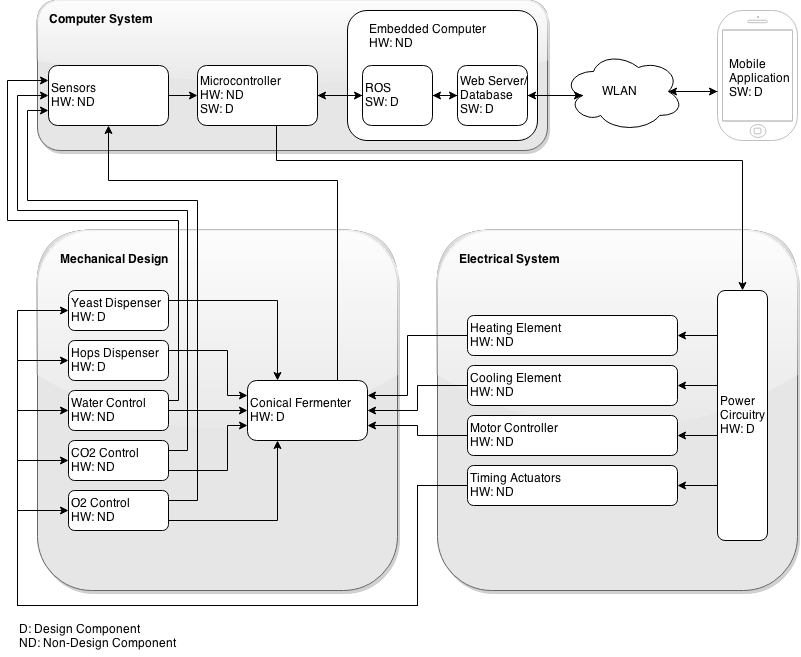
\includegraphics[scale=0.58]{block-diagram.png}
\caption{Block Diagram outlining the interactions between the computer, electrical, and mechanical systems}
\label{fig:block}
\end{center}
\end{figure}

\subsubsection{Description of System}
The single vessel brewing system, as shown in Figure \ref{fig:block}, contains various sensors which forward the environmental parameters to the microcontroller. The data from the various sensors accurately represents the state of the fermenter and feed into digital control loops running on the microcontroller.  Data from sensor modules is obtained by a microcontroller via an I2C interface. This data is then sent to an embedded computer system over USB where it is logged in a database and used to control relevant subsystems. Control commands are sent from the embedded computer to the microcontroller, where the appropriate component can be communicated with in order to regulate the brewing environment.  The embedded computer system is then able to send diagnostic information and push notifications to a mobile device through a WLAN connection.

\subsubsection{Designing and Not Designing Components}
The following is an outline of the components in the block diagram and the requirements associated for each Designing (D) and Non-Designing (ND) component.

\begin{itemize}
\item\textbf{Sensors}
\\ND: Sensors being used in the vessel are not being designed.  Instead, off-the-shelf sensors are being purchased and integrated into the system.  Relevant sensor types for this system include, but aren’t limited to, pH sensors, volume sensors, flow meters, temperature probes, etc.

\item\textbf{Microcontroller(s)}
ND: The hardware of the microcontroller is not being designed since that’s outside the scope of this project. The system instead uses an off-the-shelf microcontroller.
D: The software running on the microcontroller is being designed. This software mainly consists of digital control loops for interfacing with the sensors and power electronic circuitry.

\item\textbf{Conical Fermentation Vessel}
\\D: The mechanical features and dimensions of the conical fermentation vessel are being designed to hold various sensors and other electrical and mechanical components. 

\item\textbf{Power Electronic Circuitry}
\\D: The power electronic circuitry is being designed to power the pumps, motors, actuators, and heating/cooling mechanisms. The circuitry takes input from the digital controller running on the microcontroller and outputs the appropriate power to the end devices.

\item\textbf{Heating and Cooling Elements}
\\ND: The heating coils and refrigeration unit used to regulate temperature of the vessel are not being designed. Instead, off-the-shelf or salvaged and adapted components from existing appliances (e.g. hot water tank coils, home air conditioning heat pump) are being used and the power electronic circuitry is being designed to power these devices.

\item\textbf{Motor Controller}
\\ND: The motors, pumps, and mixing mechanisms used in our system are not being designed. Instead, off-the-shelf or salvaged and adapted components from existing appliances (e.g. blender mixing prop, aquarium pumps) are being used and the power electronic circuitry is being designed to power these devices.

\item\textbf{Timing actuators}
\\ND: The actuators used in our system are not being designed. Instead, off-the-shelf solenoids and servo motors are being used and the mechanical subsystems that they will actuate are being designed. The power electronic circuitry is also being deigned to be able to power the actuators.

\item\textbf{Embedded Computer System}
\\ND: The hardware and operating system of the embedded computer system is not a design objective as it is outside the scope of this project. Instead an off-the-shelf embedded computer is purchased and a Debian based Linux operating system is installed to satisfy the requirements for the development environment.
\\D: The embedded computer system is configured with a Web Server, Database, and the Robotics Operating System (ROS).  Microcontrollers can be modularly added to the system via USB and automatically configured as ROS nodes through negotiations.

\item\textbf{Mobile Application}
\\D: The mobile application is designed such that the user can receive push notifications and see various sensor data during the brew process.
\end{itemize}

\section{Project Specifications}
This section outlines the functional and non-functional requirements of the project design.
\subsection{Functional Specifications}
Table \ref{tab:func} describes each functional requirement and highlights whether it is essential or not to the completion of the project.

\newcolumntype{Z}{>{\raggedright\arraybackslash}X}
\begin{table}[H]
\centering
\begin{tabularx}{\textwidth}{l l Z}
\toprule
\textbf{Specification} & \textbf{Classification} & \textbf{Description} \\ 
\midrule
Completion of the Brewing Process
& Essential	
& The device automatically completes the brewing process, consisting of these steps:
\begin{itemize}
\item \Gls{mash}
\item \Gls{sparge}
\item Boil \Gls{wort}
\item Dispense Hops
\item Aerate the \Gls{wort}
\item \Gls{pitch} the Yeast
\item Kegging and Dispensing
\end{itemize}
\noindent in its entirety and in the correct order.  For more information on the brewing process and the terms used, please see the Glossary.
\\\\
Heating Unit
& Essential
& Mashing the grains, sparging the \gls{grist}, and boiling the \gls{wort} all require high water temperatures. The system is able to accurately heat the contents to a minimum of 110$^{\circ}$C within 1$^{\circ}$C of error.
\\
\end{tabularx}
\end{table}

\begin{table}[H]
\centering
\begin{tabularx}{\textwidth}{l l Z}
Cooling Unit
& Essential
& Yeast pitching and fermentation happen immediately after boiling the wort, but require temperatures a specific temperature (typically 20$^{\circ}$C). The system is able to rapidly cool the wort to a temperature within 1$^{\circ}$C of the target temperature so that the yeast may be pitched safely.
\\\\
Temperature Regulation
& Essential
& The system is able to control temperature for each step in the brewing process.  An error of 1$^{\circ}$C is the target specification.
\\\\
\Gls{trub} Removal
& Non-Essential
& Remove the undesired sediment and other byproducts at the bottom of the fermenter so that ageing may take place within the vessel.  The user does not have to maintain the \gls{trub} accumulated by the brewing process.
\\\\
Application Notifications
& Non-Essential
& The system provides notifications to the user updating them on the current state or action being taken.  Additionally errors or warnings can be sent, in cases of emergency such as clogs, low oxygen or carbon dioxide, or an improper environment.
\\\\
Database
& Essential
& The system is able query the specific steps it needs to automate for a specific brew.  Additionally, it can store various data involved in brewing including temperature, pH levels and density measurements to generate logs and reports.
\\\\
Reproducibility
& Non-Essential
& The system is able to record recipes, ingredients and steps for various brews. The user can recreate the same type of brew if they select one of the recipes.
\\
\bottomrule
\end{tabularx}
\caption{An overview of each functional specification of the project}
\label{tab:func}
\end{table}

\pagebreak
\subsection{Non-Functional Specifications}
Table \ref{tab:non-func} describes each non-functional requirement and highlights whether it is essential or not to the completion of the project.

\begin{table}[H]
\centering
\begin{tabularx}{\textwidth}{l l Z}
\toprule
\textbf{Specification} & \textbf{Classification} & \textbf{Description} \\ 
\midrule
Temperature Accuracy
& Essential
& The system accurately regulates the temperature required for the brewing process within 1$^{\circ}$C of the targeted temperature.
\\\\
Volume Control
& Essential
& The end result must be greater than or equal to the target yield volume.  Target yields typically consist of 15.5 gallons, 7.75 gallons, and 5.16 gallons.  These are the standard sizes of a half barrel keg, quarter barrel keg, and a sixth barrel keg respectively.
\\\\
Size
& Essential
& The dimensions are limited such that the vessel can fit within a standard 36 inch residential door frame.
\\\\
Mobility
& Essential
& The system is able to be relocated by a single person using the aid of caster wheels and or a standard 18 inch wide utility dolly.
\\\\
Sanitation
& Essential
& The system employs SUS 304 stainless steel to maintain food-grade sanitation conditions.  The vessel is self cleaning since a sanitary environment is crucial for the brewing process.
\\
\bottomrule
\end{tabularx}
\caption{An overview of each non-functional specification of the project}
\label{tab:non-func}
\end{table}
\pagebreak
\section{Risk Assessment}
Table \ref{tab:risk} describes each risk associated with the project and highlights methods and actions to take to mitigate any adverse effects.

\begin{table}[H]
\centering
\begin{tabularx}{\textwidth}{Z l l Z}
\toprule
\textbf{Risk} & \textbf{Impact} & \textbf{Probability} &\textbf{Mitigation} \\ 
\midrule
Funding this project proves costly and infeasible due to the requirement of expensive components
& High
& High
& Sources of additional funding and sponsorship are being investigated at an early stage of this project to mitigate this risk.
\\\\
The on-campus machine shops have insufficient manufacturing capability and precision to create the conical vessel
& High
& Medium
& Communications with the on-campus machine shop is happening at an early stage of the project, so that if necessary there is time to investigate alternative manufacturers.
\\\\
Latencies in the supply chain caused by shipping overseas cause crucial parts to arrive too close to the prototype deadline
& High
& Low
& Local suppliers for necessary parts and components are being considered first before any overseas suppliers.
\\\\
Poor quality or malfunctioning sensors cause unreliable control of the brewing process
& Medium
& High
& The use of higher quality sensors or multiple redundant sensors can lower this risk.
\\
\bottomrule
\end{tabularx}
\caption{An overview of each risk associated with the project}
\label{tab:risk}
\end{table}

\pagebreak
\printglossary[type=main]

\bibliography{specifications-bib}{}
\bibliographystyle{ieeetr}

\end{document}